\documentclass[sigconf]{acmart}

\usepackage{graphicx}
\usepackage{hyperref}
\usepackage{todonotes}

\usepackage{endfloat}
\renewcommand{\efloatseparator}{\mbox{}} % no new page between figures

\usepackage{booktabs} % For formal tables

\settopmatter{printacmref=false} % Removes citation information below abstract
\renewcommand\footnotetextcopyrightpermission[1]{} % removes footnote with conference information in first column
\pagestyle{plain} % removes running headers

\newcommand{\TODO}[1]{\todo[inline]{#1}}

\begin{document}
\title{Big Data Analysis in Finance Sector}


\author{Dhanya Mathew}
\orcid{HID328}
\affiliation{%
  \institution{Indiana University}
  \streetaddress{711 N Park Ave}
  \city{Bloomington} 
  \state{Indiana} 
  \postcode{47408}
}
\email{dhmathew@iu.edu}

% The default list of authors is too long for headers}
\renewcommand{\shortauthors}{B. Trovato et al.}


\begin{abstract}

Big data as the name implies, refers to large and complex data which continues to grow enormously day by day. The broad proliferation of data and new and efficient technological support has transformed the way industries operate and compete. Industries like financial firms, in particular, have widely adopted big data analytics to obtain better investment decisions with consistent growth. In order to understand what drives profit in an organization or company, we should be able to predict the business trends, challenges, opportunities risks and what profit group (extremely unprofitable, average, extremely profitable etc.) a set of customers falls into based on their data at any given time. Financial firms like banks are storing these data for many decades and the recent technology boom that happened with big data technologies help the firms to uncover the secrets to understand consumer behavior, prevent major disasters and theft. We show the wide possibilities open for financial firms by analyzing big data to improve decision making, productivity, customer satisfaction etc which in turn beneficial for both organizations and customers.
\end{abstract}

\keywords{i523, HID328, big data, data-driven, data lakes, Hadoop, Random Forest}


\maketitle

\section{Introduction}

There are 3 fundamental elements to big data - Volume, Variety and Velocity. Data is stored and analyzed at a speed which is nothing but the velocity\cite{how-big-data-has-changed-finance}. Data is getting increasingly gathered by low-cost and innumerable information-sensing Internet of Things devices like radio-frequency identification (RFID) readers, aerial (remote sensing), wireless sensor networks, cameras, software logs, microphones etc and hence causing data sets to grow rapidly\cite{wiki-bigdata}. Ben Walker of Voucher Cloud came up with a big data info graphic in 2015. According to Ben, the data generation per day is around 2.5 Quintillion Bytes and it would measure the height of 4 Eiffel Towers if it was stored in Blu-ray discs stacked on one another. Ben suggests that data generation by 2018 will be 50,000 GB per second\cite{how-much-data-is-created-daily}. 

According to Gartner Survey held in 2013, 64 percent of organizations were planned to invest or already invested in big data technology (including but not limited to Hadoop, NoSQL, Spark, R and Storm)\cite{gartner-survey}. Recent survey research indicates that 71 percent of firms in the financial services
industry at a global level are exploring Big
Data and predictive analytics\cite{accenture-next-generation-financial}. This number continues to grow and sectors like government, business, technology, universities, health-care, finance, manufacturing etc make use of big data to obtain meaningful information using big data technologies\cite{wiki-bigdata}. We investigate in particular, how big data is helpful in financial firms in terms of predictive analysis and profitable growth. The finance sector also contributes to the daily data generation from products and marketing, banking, business, share market etc. Finance is a very sensitive field and any useful insight can make a positive impact on the overall turnover. Historic data analysis and real time data analysis are equally important in terms of finance sector. The key idea behind is how to retrieve the 'signal' of relevant information form the bulk of data. Let us explore the wide range of possibilities of big data analysis that finance sector can come up with including decision making, discovery of new business opportunities, enhanced productivity and efficiency, risk management, fraud detection, innovation possibilities, efficiency and growth and customer segmentation.

\subsection{Efficient Decision Making}

The era of big data helps financial firms to take quality business decisions related to expanding revenues, managing costs, hiring resources etc. based on effective data analysis which provide access to real-time insights.  Data-driven decision making is one of the key advantages of big data technologies. Data driven decision making approach includes data storage, data elaboration, data analysis and decision making\cite{accenture-next-generation-financial}.

\begin{figure}[htb]
  \centering
  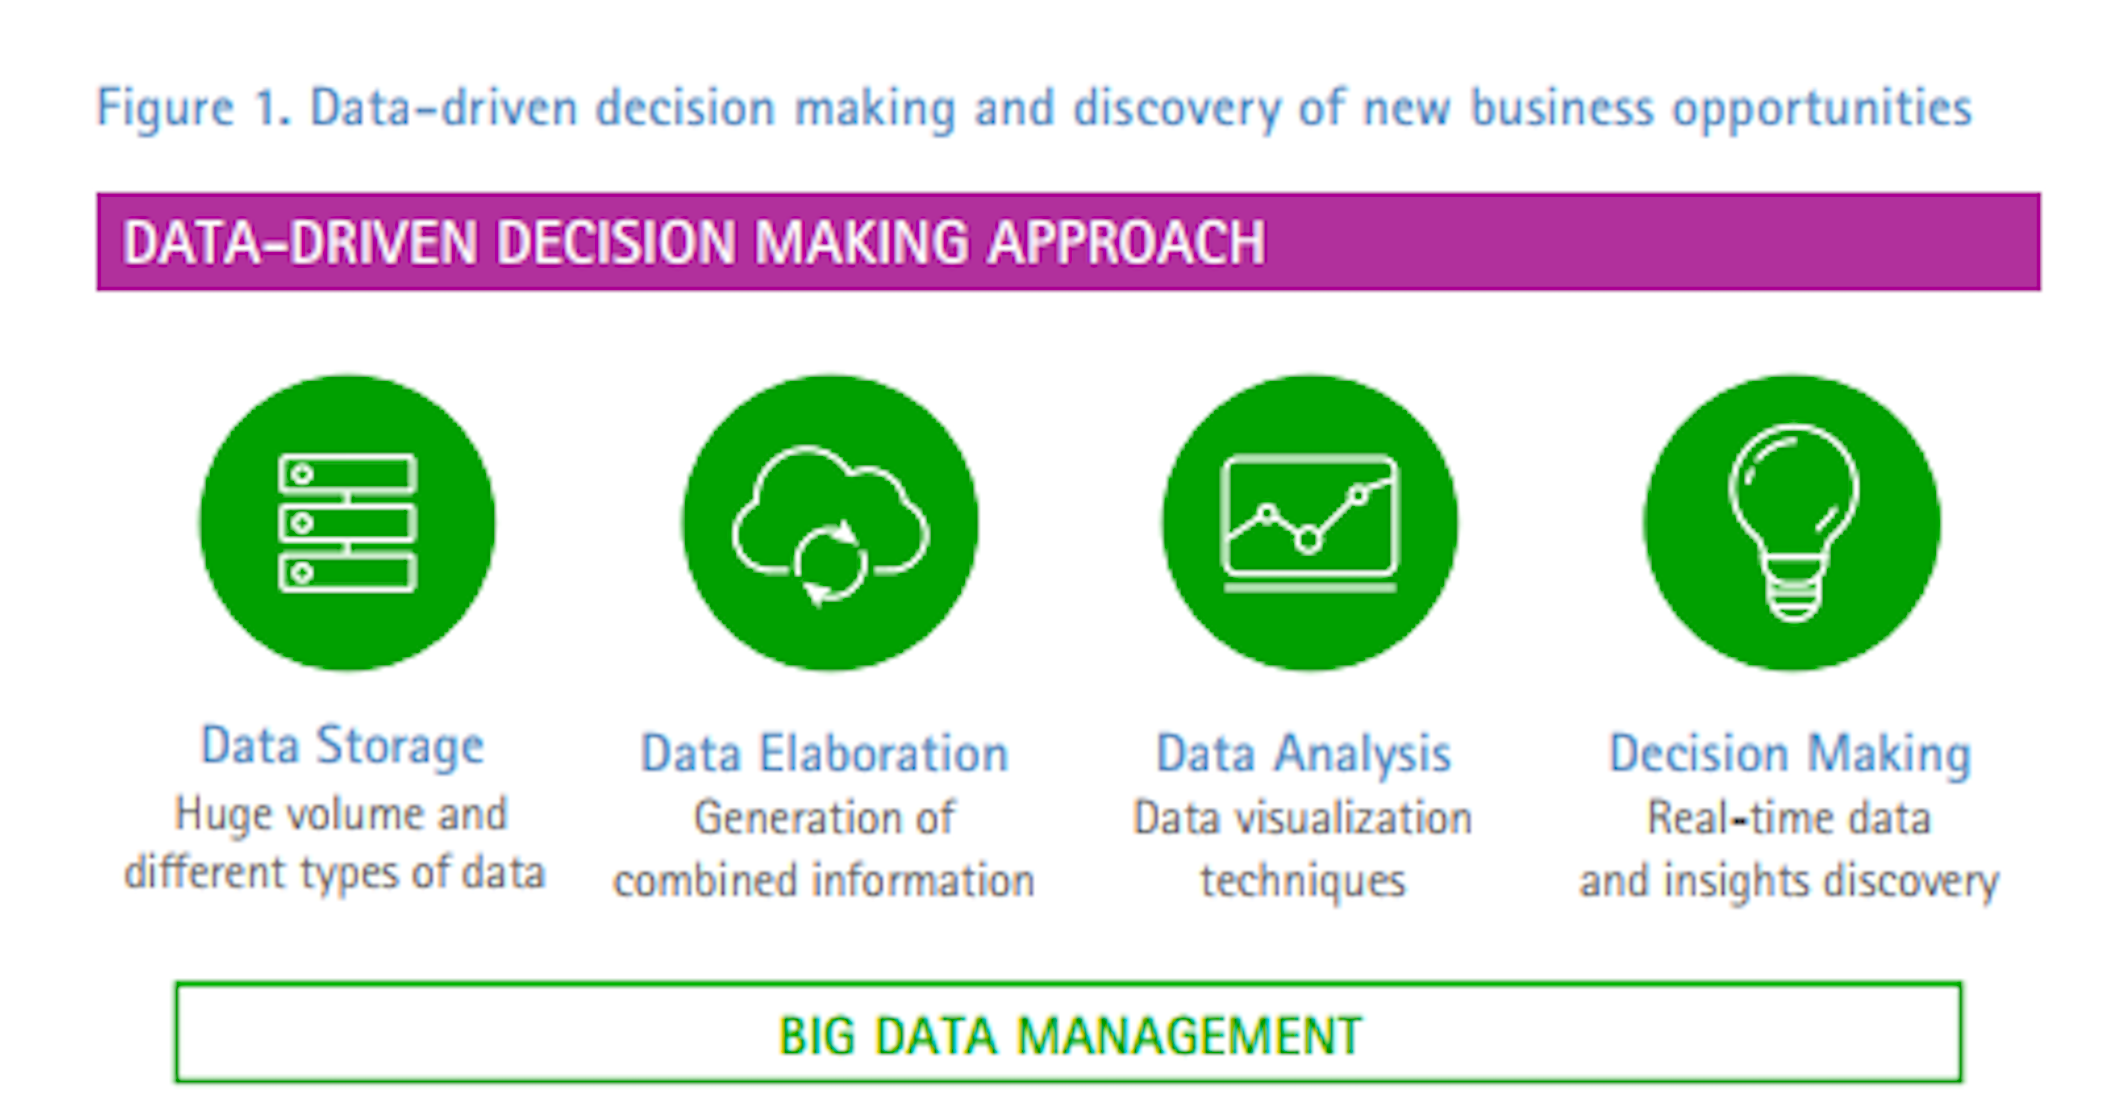
\includegraphics[width=1.0\columnwidth]{images/Figure1.png}
  \caption{Data-driven decision making approach 
  \cite{accenture-next-generation-financial}}
  \label{fig:Figure1} 
\end{figure}

Figure \ref{fig:Figure1} shows data-driven decision making approach and discovery of new business opportunities.

\textit{Data Storage:} Even though big data does not define by the size alone, we need the right means to store the huge volume and variety of data. Big data is distributed - stored across many machines and managed with Hadoop File System and distributed DBs like HBase and Apache Cassandra\cite{big-data-storage}.

\textit{Data Elaboration:} Generate combined information by eliminating unwanted data using data cleansing methods like grouping, joining, filtering etc.(Spark, R, MapReduce, Storm). 

\textit{Data Analysis:} Big data analysis is the process of analyzing the data to derive the semantics of the available data to understand the hidden patterns, correlations, market trends, customer preferences which helps the organizations to take more informed decisions. Visualization tools include- Tableau, Google chart, D3, Fusion chart etc. are used to visualize the results of analysis.

\textit{Decision Making:} Data-driven decision making based on the analysis.
 
 There is a feedback analysis done for a bank as part of 2nd International Symposium on Cloud Computing and Big Data. For an organization, feedback processes are very important. This will help the organization to recognize the potential areas of improvement and also to identify gaps in services offered if done at regular intervals. This unnamed bank also participated in a feedback process. They collected the feedback over a period of 3 years and 6 months. They gathered the data from customers visited the bank branches and online users. Customers were given a feedback survey form. They were asked to rate on a scale of 1 to 5 on the below parameters. They could do this anonymously. 
 
\begin{itemize}
   \item Whether he/she is satisfied with the services quality?
   \item Whether customer is satisfied with the turn around time?
   \item Whether the customer queries are effectively addressed?
\end{itemize}

An analysis was performed on the feedback collected from around 20,000 customers. This is actually only a subset of the actual data collected\cite{bigdata-banking}. 

\begin{figure*}[htb]
  \centering
  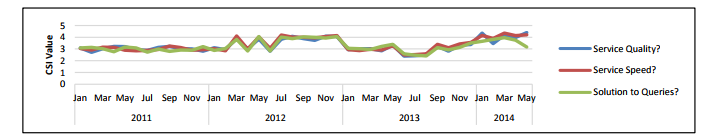
\includegraphics[width=1.0\textwidth]{images/Figure2.png}
  \caption{Overall Customer Feedback for provided parameters 
  \cite{bigdata-banking}}
  \label{fig:Figure2} 
\end{figure*}

As shown in Figure \ref{fig:Figure2}, the bank got an average rating on services offered. After that, Bank took some drastic measures to rectify the issues. This resulted in improvements in customer ratings.

\subsection{Increased Productivity and Growth}
Compared to traditional data warehouses, the big data concept of Data lakes to store raw data offers more flexibility in data access and analysis. Large volumes of data are stored, managed and analyzed in data lakes  by using automated and sophisticated analytical tools. 

Applications like, Machine learning algorithms, In-memory technologies, fast access DBs, big data queries and real-time analysis methods consume less time to come up with meaningful information and reports by accessing data lakes.

\textit{Data Lakes:} Data Lakes can be compared to the actual lakes where rivers or streams that bring water to it. In data lakes, this is called ingestion of data. We collect all the data that we require to analyze to reach our goal irrespective of the source. These 'streams' of data come in several formats: structured data (simply said, data from a traditional relational database or even spreadsheet: rows and columns), unstructured data (social, video, email, text etc.), data from all sorts of logs (weblogs, clickstream analysis etc.), XML, machine-to-machine, IoT and sensor data. Logs and XML are also called semi-structured data. There can be data filters in place based on the requirements\cite{data-lakes}.

\subsection{Fraud Detection}
One of the best ways to fight cybercrime is with early detection. Banks are prime targets for cybercriminals and fraudsters, and any kind of public breach creates a lot of embarrassment, bad publicity, and unwanted scrutiny. Clearly banks have a vested interest in any technology to identify and prevent a data breach or fraud\cite{the-top-5-trends-for-big-data-in-financial-services}.

Financial institutions use analytics to identify fraudulent transactions from the genuine ones. Analysts can identify normal behavior based on the customer's past transactions. By applying analytics and machine learning, they can easily identify a fraud transaction based on the unusual behavior.
An analysis system can have automated responses such a fraudulent transactions, including blocking that particular transaction. This stops the fraud even before it occurs. This can improve customer satisfaction and profitability of the bank\cite{5-big-data-use-cases-in-banking-and-financial-services}.

A Security and Fraud analysis was done as part of the  2nd International Symposium on Big Data and Cloud Computing. Fraud analysis coupled with behavior analysis with past transactions and customers consumption capacity will reveal a potential threat to bank and as well as uncover past frauds\cite{bigdata-banking}. 

\begin{figure}[htb]
  \centering
  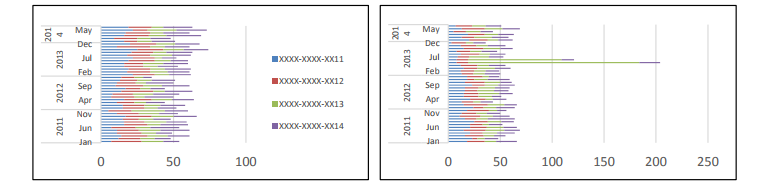
\includegraphics[width=1.0\columnwidth]{images/Figure3.png}
  \caption{Net credit transactions count 
  \cite{bigdata-banking}}
  \label{fig:Figure3} 
\end{figure}

\begin{figure}[htb]
  \centering
  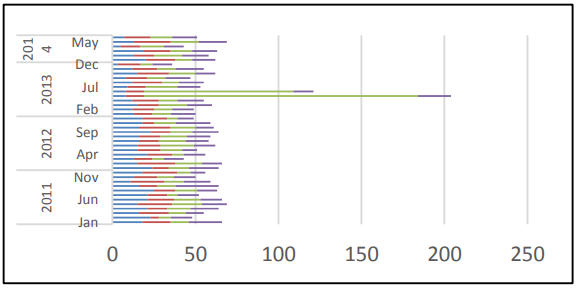
\includegraphics[width=1.0\columnwidth]{images/Figure4.png}
  \caption{Net debit transactions count
  \cite{bigdata-banking}}
  \label{fig:Figure4} 
\end{figure}

As shown in Figure \ref{fig:Figure3}, the credit card transactions per card are increasing with time and the net ratio with previous month is the same.
From Figure \ref{fig:Figure4}, we can notice that, in the month of May and June 2013, card number ending 13 shows a spike in transaction count. The transactions are doubled during the said period for this particular card. Ideally, an analyst should sound an alarm in this particular case. When we upscale to include millions of customers, such spikes are dangerous. This means a potential system compromise. This clearly indicates a misuse of the card and unauthorized access of funds by frauds.



\subsection{Customer Segmentation and Personalized Marketing}

Customer segmentation helps banks to transform from product-centric to customer-centric business. Big data enables the bank to group customers into segments. Customer segments are derived from the data sets. The dataset includes demographics, transactions, interactions with online and telephone customer services. And also external data, such as housing price. Financial institutions can then run targetted campaigns based on this segments\cite{5-big-data-use-cases-in-banking-and-financial-services}.

There are many segmentation identification algorithms available in the Big Data world.  Random Forest is one of the prominent algorithm. Apache spark, R are some of the technologies that have good integration with segmentation algorithms

\textit{Personalized Marketing:} Using big data technologies, financial services firms can analyze their customer's merchant records and social media profiles to get a complete picture of their needs.  This kind of marketing is done primarily by understanding customer's individual buying habits. It is beyond segment-based marketing and is called personalized marketing. Once those needs are understood, big data analysis can create a credit risk assessment in order to decide whether or not to go ahead with a transaction\cite{5-big-data-use-cases-in-banking-and-financial-services}.

    
\subsection{Understand New Business Opportunities}
Big data will essentially change the manner in which business operate and compete. Institutions that are heavily invested in the big data space will have an identifiable advantage over others. As more and more data is generated, a performance gap will continue to grow. Emerging technologies ( enable faster and easier data analysis) and digital channels will help them to offer better solutions. It is difficult to identify what is most important in the data, which technologies best suits the needs, who the customers are and what they expect. Being more data-driven gives an edge over competitors\cite{bigdata-ey}.

Big data incorporated with data science and business strategy can provide significant competitive advantages to organizations by offering new business opportunities. It allows companies to equip the data with pertinent real-time information when making decisions in order to eliminate inefficient operating processes, enhance the customer experience, take advantage of new markets, etc. For many companies and businesses, big data is already a critical path to develop new products, services and business models\cite{accenture-next-generation-financial}.

\subsection{Discovery of Innovation Possibilities}
Data analysis is increasingly becoming a key differentiator between wildly profitable and struggling businesses. Exploring and analyzing data, translates information into insight and drives to innovations\cite{bigdata-innovations}.

Successful firms make decisions based on facts and data rather than intuition and are open to innovation concepts. 


\subsection{Risk Management}
Financial firms especially banking sector are facing new regulatory requirements and challenges or risks each year. Big data adoption provides organizations a simplified and data-driven solution to mitigate the risks and helps to convert the data into usable information for regulatory reporting. Using data lakes and stronger analytic tools   also helps to foresee the expected impact quickly\cite{the-real-world-use-of-big-data-935}.

\subsection{Cost Effective Information Gathering}

Unlike traditional business intelligence systems, new techniques and technologies used with Big Data allow to gain useful information at a much lower cost. New architectures and the move from data silos to 'data lakes' can provide substantial cost advantages and greater scalability due to flexibility in the data analysis. In fact, having all data sources in a data lake allows users to pull new reports on relatively new data, while in traditional data warehouses (DWHs) users have to extract, transform and load (ETL) new data into a static data model, which is expensive and costly from a time perspective. By using automated and sophisticated analytical tools that can store and analyze data faster and more easily, organizations can reduce the overall cost\cite{accenture-next-generation-financial}.

\subsection{Big data - Risks and Considerations}

Big data plays an progressively important role in the financial services sector. It is used for every single thing from targeting advertisements to optimizing portfolios. While these technologies have many benefits, critics are quick to point out that they can also become a source of discrimination if they are developed and/or used in an improper way\cite{risk-with-bigdata}.

\textit{Data Security:} When we are considering the logistics of data collection and analysis, concern about data security is obvious and often takes top place in our mind. Data theft is an uncontrolled and growing area of crime. Security-related attacks are getting wider and more damaging\cite{5risks-bigdata}.

\textit{Data Privacy:} Data privacy is closely related to the issue of data security. We need to ensure that people's personal data are safe from criminals. Also, it is essential to be sure that the sensitive information being collected and stored are not going to be misused by yourself or by people who are authorized to analyze and report on it\cite{5risks-bigdata}.

\textit{Bad Analytics:} Bad analytics means 'getting it wrong'. It is obviously a risk to misinterpret the data patterns shown by the data where in fact there may simply a random coincidence. For example, product sales may increase following a major sporting event. Sales data will show this rise prompting you to relate your product with sports fans. But in fact, the rise was because of more people in town. The same situation can happen after a big music event as well\cite{5risks-bigdata}.

\textit{Bad Data:} There can be scenarios where data projects start off by collecting immaterial, erroneous, or out of date data which tend to have less time in designing the project strategy\cite{5risks-bigdata}.


\section{Conclusion}
The Big Data revolution offers new opportunities for profitable growth and the financial services firms being one of the most risk-laden and dynamic of all business segments globally, are responding to it enthusiastically. It has become their derived knowledge that making sizeable investments in big data is ultimately a gain. Data has become the key element for decision making with the right choice of analytical tools and skill-set. When data from multiple sources combined and analyzed in a smart way, there emerges the insights which derive intelligent decisions and finally drives to profit.

\begin{acks}

The author would like to thank the web loaded with information on any subject. The author would also like to thank Prof. Gregor von Laszewski for his review and suggestions.

\end{acks}


\bibliographystyle{ACM-Reference-Format}
\bibliography{report} 

\end{document}
